\section{L'apodisation}

Le but de l'apodisation est de "lisser" un signal assez brut afin d'enlever ou adoucir les discontinuités sur ses bords. 
Cela va permetttre d'augmenter le contraste et de supprimer, du moins en partie, les anneaux de diffraction produits par un instrument d'optique, afin d'améliorer la définition des éléments à étudier.

\subsection{Bases sur la diffraction — Transformée de Fourier}

- La conversion pour comprendre comment on passe du plan pupille au plan focal
- graphe largeur commune et tout, avec condition que la planete soit visible a tout les longueur d’onde et que la largeur commune soit plus grand que le coeur de la PSF a la longueur d’onde max

Prenons l'exemple classique du signal d'une étoile, que l'on considèrera comme une source ponctuelle à l'infini, passant à travers l'ouverture circulaire d'un téléscope. 

On part d'une onde plane à l'infini qui passe à travers une ouverture circulaire. Lorsque l'onde atteint ce plan, elle devient alors une fonction circulaire $\text{circ}_r(\rho')$.
En passant par cette ouverture, la fonction circulaire devient par transformée de Fourier (c.f. \emph{Diffraction de Fraunhofer à l'infini}) la fonction de Bessel d'ordre 1 $J_1$ (Fig. 1.a), qu'on appelle aussi fonction "sombrero".

\begin{figure}[htbp]
    \centering
    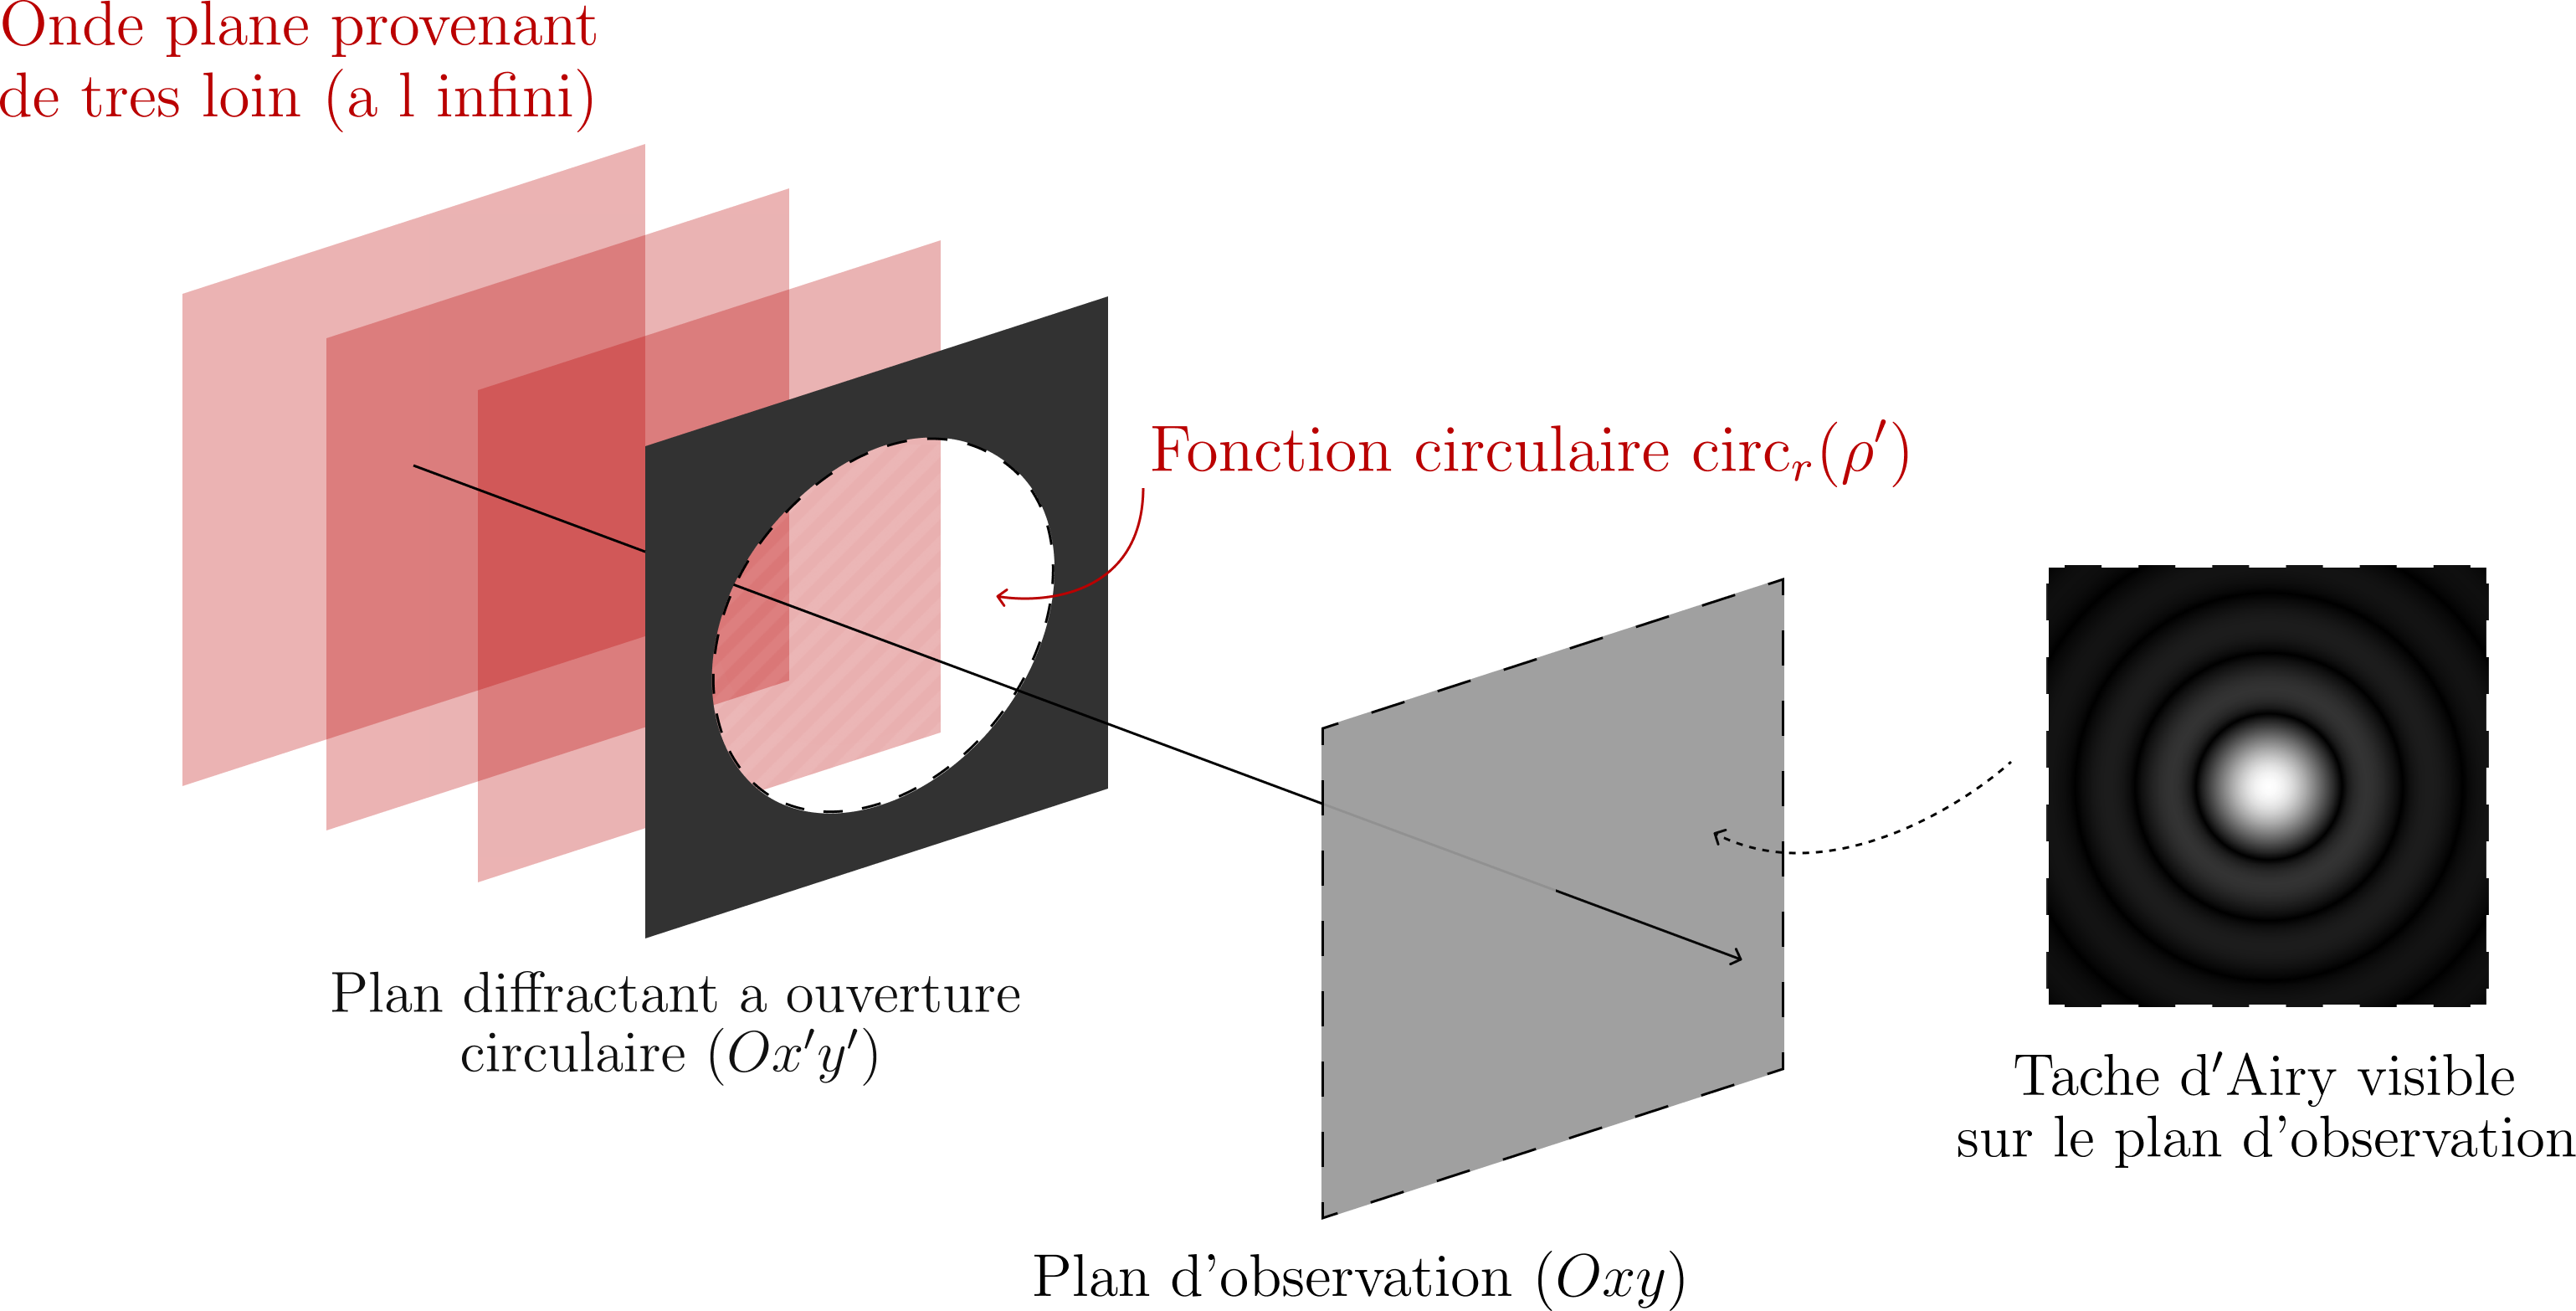
\includegraphics[width=0.75\textwidth]{figures/diff.png}
    \caption{Diffraction d'une onde plane par une ouverture circulaire.}
\end{figure}

Ce qu'on voit sur nos écrans lors des mesures est la \textbf{tâche d'Airy} (Fig 1.b), qui correspond à la fonction sombrero vue du dessus.

\begin{figure}[htbp]
    \centering
    \begin{subfigure}[b]{0.35\textwidth}
        \centering
        \includegraphics[width=\textwidth]{/Users/lalyboyer/Desktop/sombrr.png}
        \caption{Fonction de Bessel d'ordre 1 $J_1$, aussi appelé "fonction sombrero".}
    \end{subfigure}
    \hspace*{3cm}
    \begin{subfigure}[b]{0.35\textwidth}
        \centering
        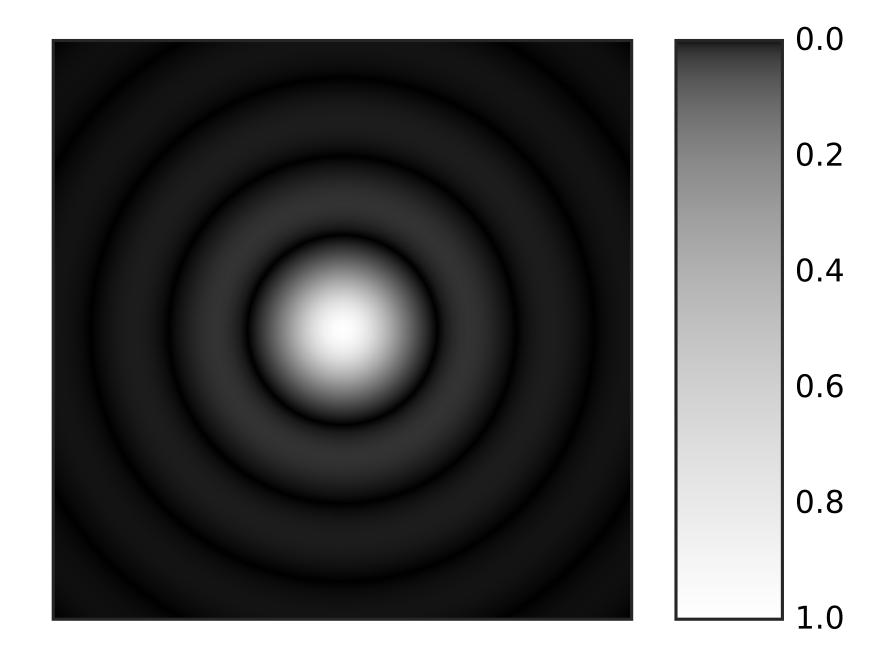
\includegraphics[width=\textwidth]{figures/airy_disk.png}
        \caption{Tâche d'Airy. L'intensité maximum de la tâche est atteinte en son centre, où est concentré la majorité de l'énergie.}
    \end{subfigure}
    \caption{Comparaison entre la fonction sombrero et la tâche d'Airy. On remarque que la tâche d'Airy correspond à la vue de dessus de la fonction $J_1$}
\end{figure}


Cette tâche d’Airy entraine toute une série d’implications pour l’imagerie, car une lentille n’est pas
infinie et limite la taille de l’onde. Cela entraine que l’image d’un point ne peut pas être un point mais
va être une tâche proportionnelle au rayon de la tâche d’Airy, ce rayon étant proportionnel à $\lambda$. %c’est ce qui explique que l’on peut mieux focaliser un laser bleu qu’un laser rouge
%et donc que le blue ray peut contenir plus d’information qu’un CD lu par un laser rouge.

Globallement, le centre de cette tâche (soit l'information compris dans le rayon $< 1.22\: \nicefrac{\lambda}{D}$) correspond à ce qu'on appelera le \textbf{coeur de la PSF} : l'essentiel de l'information qu'on peut récupérer à partir de la lumière de l'étoile se trouve dedans.



Ainsi, nous nous retrouvons à comprendre la nécessité de l'apodisation : la lumière diffracté de l'étoile va venir complétement recouvrir la lumière de l'exoplanète, rendant impossible l'analyse \iffalse ou genre récupérer l'information? \fi de la lumière de cette dernière. 

%Image montrant l'exemple

\begin{figure}[htbp]
    \centering
    \begin{subfigure}[b]{0.45\textwidth}
        \centering
        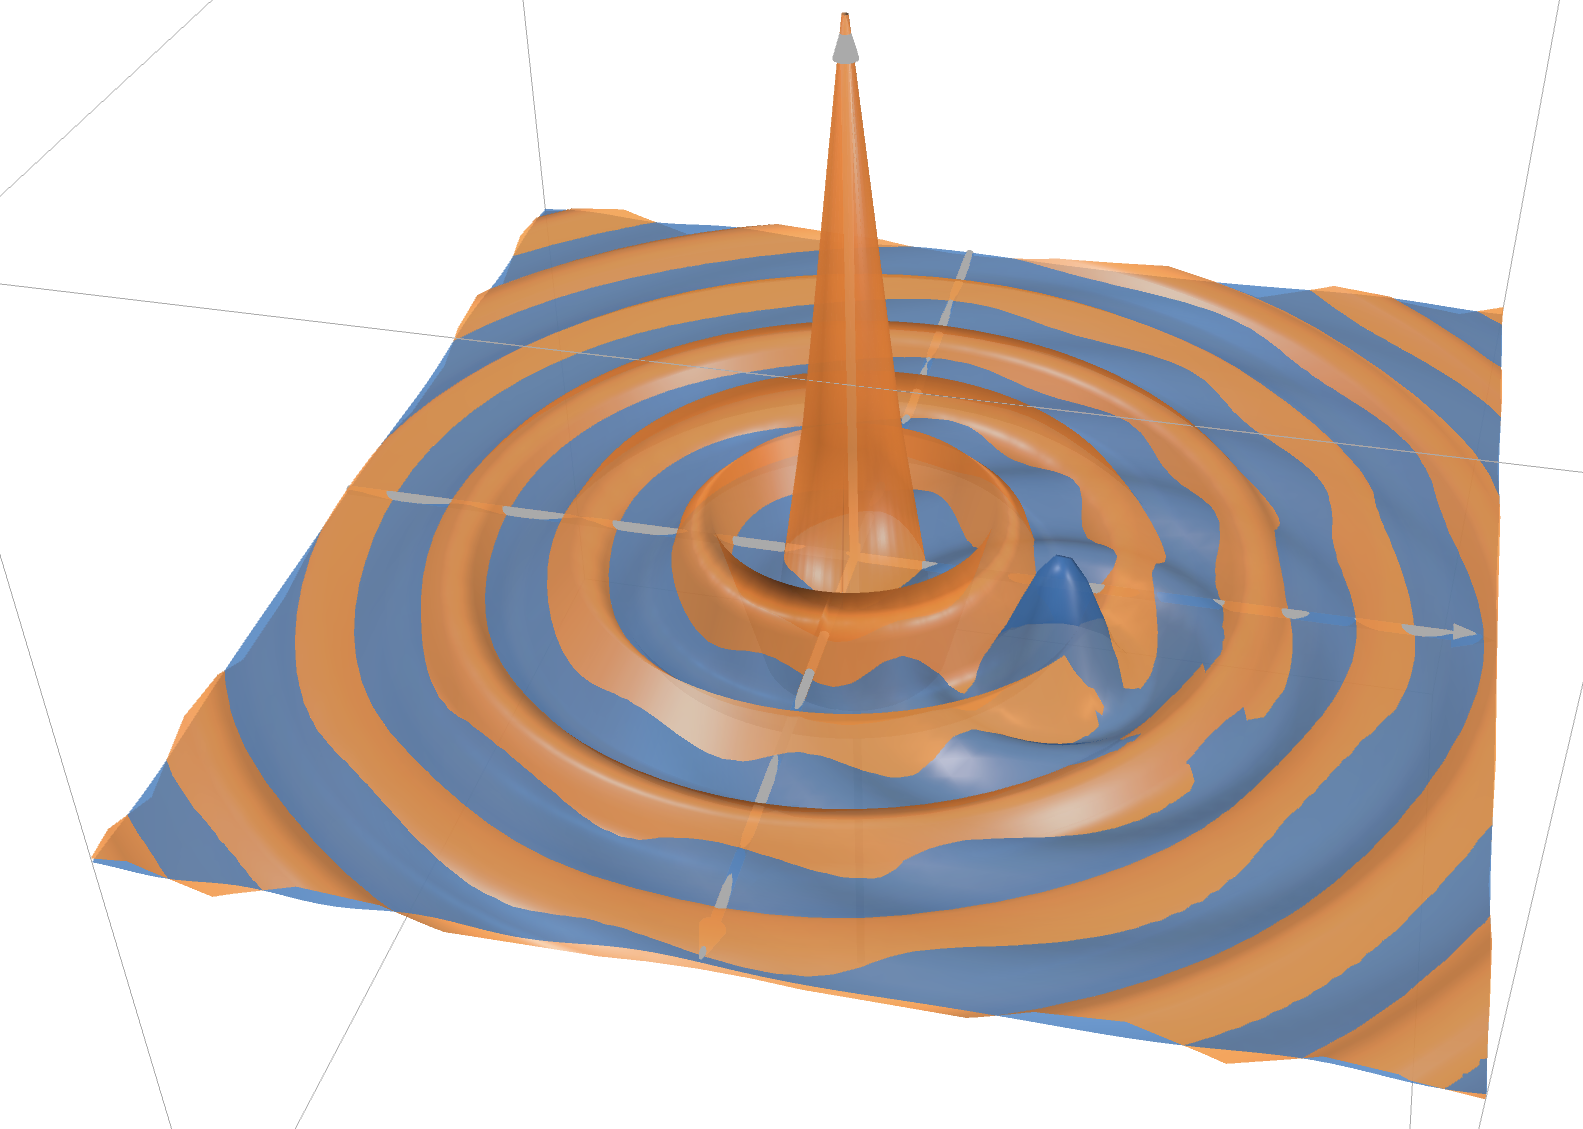
\includegraphics[width=\textwidth]{figures/st_pl_sgn.png}
        \caption{Zoomée sur la tâche d'Airy.}
    \end{subfigure}
    \hfill
    \begin{subfigure}[b]{0.45\textwidth}
        \centering
        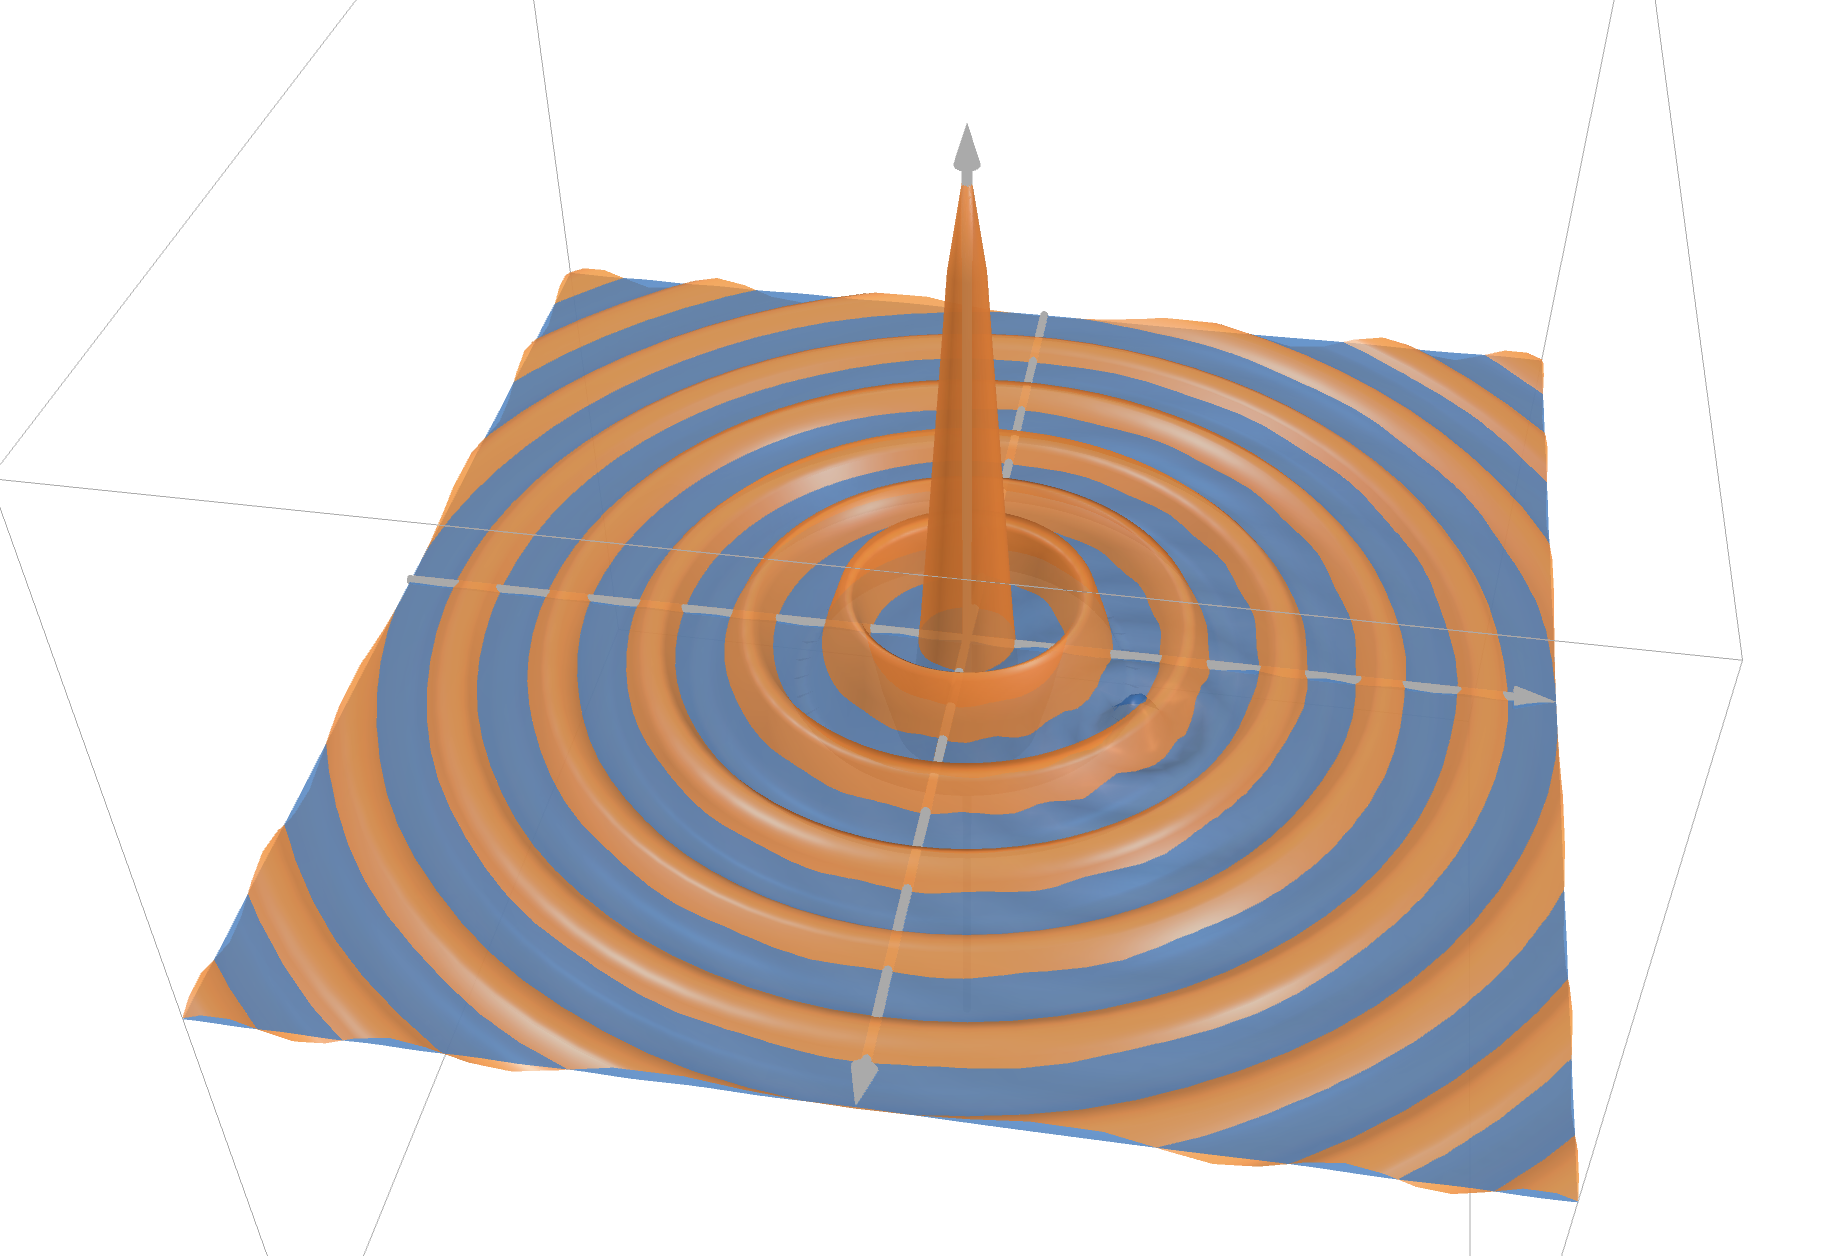
\includegraphics[width=\textwidth]{figures/larg_st_pl_sgn.png}
        \caption{Tâche d'Airy d'une exoplanète indistinguable de celle de l'étoile.}
    \end{subfigure}
    \caption{Exemple de la tâche d'Airy d'une étoile et de son exoplanète proche, avec (a) montrant un signal à peu près distinguable et en (b) le signal de l'exoplanète encore plus faible que l'exemple (a), rendant impossible la récupération de l'information de la planète.}
\end{figure}


Afin de pouvoir créer une zone de haut contraste permettant l'observation d'une exoplanète proche de son étoile, différentes méthodes sont possibles : nous choisirons ici l’apodisation à l’aide d’un \textbf{masque pupille}; nous allons commencer par définir ce dont il s'agit.

\subsection{Masque pupille — Apodiseur}

Un masque pupille (aussi appelé \emph{apodiseur}) est un carré en verre recouvert de chromium que l'on place dans le téléscope permettant de diffracter la lumière entrante dans le télescope de tel manière à pouvoir créer une zone où le contraste est suffisamment faible pour pouvoir observer des objets à luminosité très faibles autour d'objet très lumineux.

Ces masques permettent de diffracter la lumière autour de l’étoile afin de pouvoir créer une zone de haut contraste dans une zone souhaitée.

Illustration of the apodization technique in the focalplane. Top left: unapodized amplitude split into two shiftedamplitude (bottom left). The result of this coherent additionis the first-apodized amplitude (top center). This approachcan be iteratively reproduced: the split and shifted amplitudes(bottom center) and second-apodized amplitude (top right).

\begin{figure}[htbp]
    \centering
    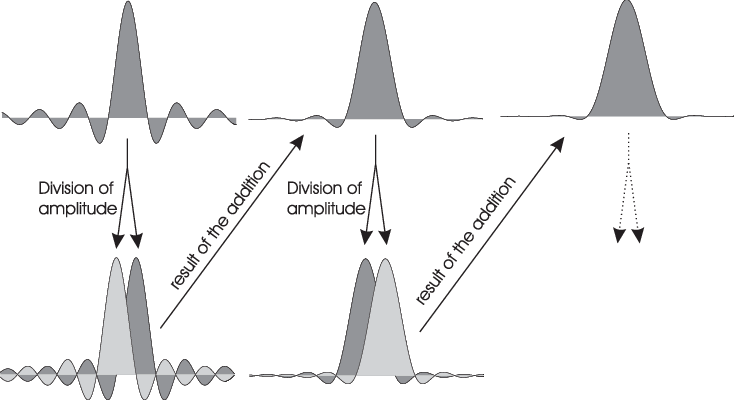
\includegraphics[width=0.7\textwidth]{figures/apod_explanation.png}
    \caption{Illustration de la technique d'apodisation dans le plan focal. En haut à gauche : amplitude non apodisée divisée en deux amplitudes décalées (en bas à gauche). Le résultat de cette addition cohérente est l'amplitude apodisée (en haut au centre). Cette approche peut être reproduite de manière itérative : les amplitudes divisées et décalées (en bas au centre) et l'amplitude apodisée (en haut à droite). }%\cite{apodExpl}}
\end{figure}

On peut ainsi remarquer qu'au fur et a mesure qu'on itère cette méthode, on crée une zone de haut contraste de plus en plus grande, permettant de récupérer de plus en plus d'information de l'exoplanète.

%Image montrant le principe physique de l'apodisation
Cependant, ce processus implique forcément une perte d'information, car la lumière de l'étoile est aussi diffractée. C'est pourquoi il est important de trouver un compromis entre la taille de la zone de haut contraste et la perte d'information.

En gros, on perd en résolution pour réduire la diffraction de l'étoile et augmenter le contraste de l'exoplanète.
% L’apodisation est une technique permettant de modifier la forme d’une fonction mathématique représentant un signal électrique, une transmission optique… de tel façon à enlever ou adoucir les discontinuités sur ces bords.
% Procédé destiné à augmenter le contraste et à supprimer, du moins en partie, les anneaux de diffraction produits par un instrument d'optique, afin d'améliorer la définition des éléments à étudier. [2.]
\begin{figure}[htbp]
    \centering
    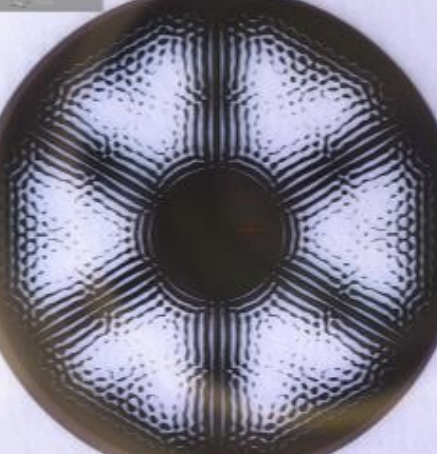
\includegraphics[width=0.4\textwidth]{figures/apod_harmoni.png}
    \caption{Apodiseur HC1 de l'instrument HARMONI.}%\cite{apod_harmoni}}
    %\label{fig:apod_harmoni}
\end{figure}
% L’apodisation est une technique permettant de modifier la forme d’une fonction mathématique représentant un signal électrique, une transmission optique… de tel façon à enlever ou adoucir les discontinuités sur ces bords.

% Procédé destiné à augmenter le contraste et à supprimer, du moins en partie, les anneaux de diffraction produits par un instrument d'optique, afin d'améliorer la définition des éléments à étudier. [2.]